\documentclass[10pt,twocolumn]{article}

\usepackage[margin=0.72in,columnsep=0.24in]{geometry}
\usepackage[T1]{fontenc}
\usepackage[utf8]{inputenc}
\usepackage{lmodern}
\usepackage{microtype}
\usepackage{amsmath,amssymb}
\usepackage{booktabs}
\usepackage{tabularx}
\usepackage{caption}
\usepackage{graphicx}
\usepackage{tikz}
\usepackage{enumitem}
\usepackage{xcolor}
\usepackage{xurl}
\usepackage{seqsplit}
\usepackage{hyperref}
\usepackage[capitalise,noabbrev]{cleveref}
\usetikzlibrary{arrows.meta,positioning,fit,backgrounds}

\definecolor{FBBlue}{HTML}{1769AA}
\definecolor{FBGold}{HTML}{E6A11A}
\definecolor{FBTeal}{HTML}{168C7A}
\definecolor{FBRed}{HTML}{C75450}
\definecolor{FBCharcoal}{HTML}{262B33}
\definecolor{FBPaper}{HTML}{F7F8FA}
\hypersetup{
  colorlinks=true,
  linkcolor=FBBlue,
  citecolor=FBBlue,
  urlcolor=FBBlue,
  pdftitle={FlavourBench: Ranking Frontier Language Models with Executable Culinary Ground Truth},
  pdfauthor={Josef Chen, Erim Hayretci},
  pdfsubject={An executable benchmark of culinary reasoning in frontier language models},
  pdfkeywords={language models, executable benchmarks, culinary reasoning, evaluation,
    statistical ranking}
}
\setlist{leftmargin=*,nosep}
\setlength{\parindent}{1em}
\setlength{\parskip}{0pt}

\newcommand{\system}{\textsc{FlavourBench}}
\newcommand{\epicure}{\textsc{Epicure}}
\newcommand{\sha}[1]{\texttt{\seqsplit{#1}}}
\newcommand{\FBModels}{27}
\newcommand{\FBTasks}{534}
\newcommand{\FBTasksPerFamily}{178}
\newcommand{\FBTasksPerPanelFamily}{89}
\newcommand{\FBPanelCount}{2}
\newcommand{\FBFamilies}{3}
\newcommand{\FBUniqueAnchors}{534}
\newcommand{\FBSelectionsPerTask}{56}
\newcommand{\FBPrefrozenScores}{29904}
\newcommand{\FBPrimaryCells}{14418}
\newcommand{\FBPairs}{351}
\newcommand{\FBSignificantPairs}{101}
\newcommand{\FBBootstrapResamples}{50000}
\newcommand{\FBPermutationResamples}{100000}
\newcommand{\FBTopModel}{Grok 4.6}
\newcommand{\FBTopScore}{65.1}
\newcommand{\FBTopCILow}{61.0}
\newcommand{\FBTopCIHigh}{69.2}
\newcommand{\FBTopGroup}{1}
\newcommand{\FBDefinitiveTop}{no}
\newcommand{\FBPanelPearson}{0.89}
\newcommand{\FBPanelSpearman}{0.80}
\newcommand{\FBIndependentClusters}{534}
\newcommand{\FBCompleteCells}{14418}
\newcommand{\FBPlanDigest}{2ba71c793c8d}


\title{\vspace{-1.4em}\system{}: Ranking Frontier Language Models with\\
Executable Culinary Ground Truth}
\author{
  Josef Chen\\[-0.1em]\small Independent Researcher
  \and Erim Hayretci\\[-0.1em]\small Imperial College London
}
\date{August 2026}

\begin{document}
\raggedbottom
\twocolumn[
  \begin{@twocolumnfalse}
  \maketitle
  \vspace{-1.1em}
  \begin{abstract}
  Open-ended language-model benchmarks usually inherit a judge: a human preference panel,
  another model, or a brittle exact-match key. We introduce \system{}, an automated benchmark in
  which a versioned culinary system supplies dense, executable ground truth. Each task presents
  eight ingredients and asks for a three-ingredient portfolio; before model execution,
  \epicure{} scores all 56 possible portfolios. We evaluate \FBModels{} frontier endpoints on an
  identical \FBTasks{}-task core spanning substitution, pairing, and constrained composition.
  Every ranked model has exactly \FBTasksPerPanelFamily{} valid responses per panel and family
  (\FBCompleteCells{} model--task cells total), eliminating differential missingness from the
  leaderboard. The FlavourBench Score is the equal-family mean of the frozen task scores. We use
  \FBBootstrapResamples{} anchor-cluster bootstrap replicates for simultaneous 95\% score bands
  and \FBPermutationResamples{} sign-flip draws for all \FBPairs{} paired model contrasts, with
  Holm control. The two independently compiled panels correlate at $r=\FBPanelPearson{}$ (rank
  $\rho=\FBPanelSpearman{}$). \FBTopModel{} has the largest point estimate at \FBTopScore{}
  (simultaneous 95\% CI \FBTopCILow{}--\FBTopCIHigh{}); \FBSignificantPairs{} of \FBPairs{}
  model pairs are resolved. The release includes the prompts, all portfolio score maps, raw
  responses, exact routes, content hashes, and an offline verifier that reconstructs every result.
  \end{abstract}
  \vspace{0.5em}
  \end{@twocolumnfalse}
]

\section{Introduction}

Benchmarks are strongest when the evaluator can be executed. Code can be tested, database states
can be inspected, and games can be scored. Culinary reasoning is usually evaluated with a model
judge, a handful of human preferences, or factual questions whose answers do not capture the
quality of a complete decision. That leaves two problems: the judge is entangled with the systems
being tested, and exact match throws away useful differences between plausible answers.

\system{} turns a culinary runtime into a benchmark environment. \epicure{} represents 1,790
ingredients in a 300-dimensional space and exposes deterministic operations for substitution,
pairing, dietary feasibility, and regional composition
\cite{radzikowski2026structure,radzikowski2026geometry}. A task compiler converts these operations
into three-of-eight selection problems. It enumerates every candidate portfolio and freezes a
continuous 0--100 score map before model execution. An answer is therefore scored by table lookup,
without a model judge and without post-hoc interpretation.

This setup separates the reference system from the evaluated systems. \epicure{} is not a
leaderboard entry and is not ``100\% accurate.'' It defines the task-specific reward surface. A
model receives 100 on a task only if it selects that task's highest-scoring portfolio; other valid
portfolios receive partial credit. The benchmark measures agreement with a published executable
culinary environment, not universal human taste.

We use that environment to evaluate \FBModels{} current endpoints. Every model faces the same
\FBTasks{} tasks and \FBSelectionsPerTask{} frozen answer scores per task. The complete common core
supports direct paired comparisons on \FBTasks{} shared observations per model pair instead of
inferring a ranking from sparse votes or comparing endpoints on different task subsets.

The paper makes three contributions:
\begin{enumerate}[label=\arabic*.]
  \item an executable culinary benchmark with \FBPrefrozenScores{} model-independent portfolio
  scores and a single interpretable 0--100 metric;
  \item a \FBModels{}-model, \FBTasks{}-task complete-core evaluation with simultaneous
  uncertainty and paired, multiplicity-controlled tests; and
  \item a content-addressed release in which every public number traces to frozen tasks, exact
  routes, raw responses, and a dependency-light offline scorer.
\end{enumerate}

\begin{figure*}[t]
  \centering
  \resizebox{\linewidth}{!}{%
  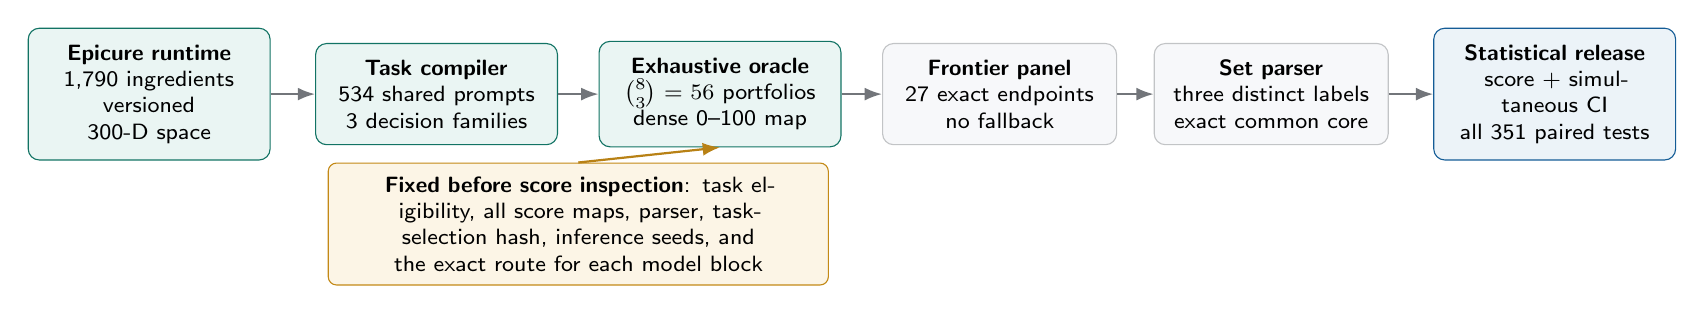
\begin{tikzpicture}[
    x=1cm,y=1cm,font=\sffamily\footnotesize,
    box/.style={draw=FBCharcoal!28,rounded corners=4pt,fill=FBPaper,
      minimum height=1.25cm,text width=2.55cm,align=center,inner sep=6pt},
    oracle/.style={draw=FBTeal!82!black,rounded corners=4pt,fill=FBTeal!9,
      minimum height=1.25cm,text width=2.65cm,align=center,inner sep=6pt},
    score/.style={draw=FBBlue!88!black,rounded corners=4pt,fill=FBBlue!8,
      minimum height=1.25cm,text width=2.65cm,align=center,inner sep=6pt},
    arrow/.style={-{Latex[length=2.2mm]},thick,draw=FBCharcoal!65}
  ]
    \node[oracle] (runtime) at (0,0) {\textbf{Epicure runtime}\\1,790 ingredients\\versioned 300-D space};
    \node[oracle] (compiler) at (3.65,0) {\textbf{Task compiler}\\\FBTasks{} shared prompts\\3 decision families};
    \node[oracle] (enumerate) at (7.25,0) {\textbf{Exhaustive oracle}\\$\binom{8}{3}=56$ portfolios\\dense 0--100 map};
    \node[box] (models) at (10.8,0) {\textbf{Frontier panel}\\\FBModels{} exact endpoints\\no fallback};
    \node[box] (parser) at (14.25,0) {\textbf{Set parser}\\three distinct labels\\exact common core};
    \node[score] (inference) at (17.85,0) {\textbf{Statistical release}\\score + simultaneous CI\\all 351 paired tests};

    \draw[arrow] (runtime) -- (compiler);
    \draw[arrow] (compiler) -- (enumerate);
    \draw[arrow] (enumerate) -- (models);
    \draw[arrow] (models) -- (parser);
    \draw[arrow] (parser) -- (inference);

    \node[draw=FBGold!85!black,rounded corners=3pt,fill=FBGold!11,
      text width=6.0cm,align=center,inner sep=5pt] (freeze) at (5.45,-1.65)
      {\textbf{Fixed before score inspection}: task eligibility, all score maps, parser,
      task-selection hash, inference seeds, and the exact route for each model block};
    \draw[arrow,draw=FBGold!80!black] (freeze.north) -- (enumerate.south);
  \end{tikzpicture}}
  \caption{\system{} compiles a versioned culinary runtime into dense selection tasks. The
  evaluated models never judge one another and do not access \epicure{}. All score maps and the
  per-panel contracts are fixed before collection. The complete-core task set is selected from
  response validity alone, before inspecting any model selection or score.}
  \label{fig:architecture}
\end{figure*}

\section{Executable culinary ground truth}
\label{sec:ground-truth}

\subsection{A reference environment, not a model judge}

The benchmark binds an exact \epicure{} release, evidence bundle, application build, ingredient
count, and embedding dimensionality by hash. Changing any of these inputs creates a new benchmark
task-set identity. This is analogous to fixing a simulator or a code-test suite: the reference is
explicit and reproducible, but its external validity remains a scientific question rather than an
assumption hidden inside a judge prompt.

For each task $t$, let $\mathcal{A}_t$ contain all 56 three-item subsets of eight candidates.
\epicure{} assigns a raw utility $u_t(a)$ to every valid $a\in\mathcal{A}_t$. Invalid portfolios
under a dietary or category constraint receive zero. Valid utilities are normalized within the
task:
\begin{equation}
 s_t(a)=100\,\frac{u_t(a)-\min_{b\in\mathcal{A}_t}u_t(b)}
 {\max_{b\in\mathcal{A}_t}u_t(b)-\min_{b\in\mathcal{A}_t}u_t(b)}.
 \label{eq:task-score}
\end{equation}
Every task has a unique 100-point optimum. The exact chance baseline is not a generic percentage;
it is $|\mathcal{A}_t|^{-1}\sum_a s_t(a)$ for that frozen task.

\subsection{Three complete-core decision families}

The ranked core contains \FBTasks{} tasks: \FBTasksPerPanelFamily{} from each family in each of two
independently compiled panels, spanning \FBUniqueAnchors{} unique anchor ingredients. Tasks sharing
an anchor move together as one cluster in inference. Candidate sets are selected across validation
strata, then ordered and labeled by a task-derived hash. No evaluated model writes an item,
distractor, or score. Regional-composition tasks are released as a supplemental track but are not
in the 27-model leaderboard because they do not support an equally complete common core.

\begin{table*}[t]
  \centering
  \footnotesize
  \setlength{\tabcolsep}{4pt}
  \begin{tabularx}{\linewidth}{@{}l X X X r@{}}
    \toprule
    Family & Decision & Epicure utility & Hard constraint & Tasks \\
    \midrule
    Substitution & choose a three-item replacement portfolio for an anchor ingredient &
      $0.8$ anchor similarity $+0.2$ portfolio coherence & none & \FBTasksPerFamily{} \\
    Pairing & choose three ingredients to accompany an anchor &
      $0.65$ anchor affinity $+0.35$ portfolio coherence & none & \FBTasksPerFamily{} \\
    Constraints & choose a feasible portfolio under diet and processing limits &
      $0.7$ anchor similarity $+0.3$ coherence & diet and maximum NOVA level & \FBTasksPerFamily{} \\
    \bottomrule
  \end{tabularx}
  \caption{The three complete-core task families share one response and scoring interface but
  probe different culinary decisions. Each task contains eight candidates and 56 frozen scores.}
  \label{tab:task-families}
\end{table*}

The score maps have substantial resolution rather than one correct key plus 55 equivalent
mistakes. \Cref{tab:task-diagnostics} reports the exact random-portfolio baseline, separation of
the best and second-best portfolios, and the number of distinct score values. Constraint tasks are
intentionally sparse because infeasible portfolios score zero; the other families provide much
finer graded rewards.

\begin{table}[t]
  \centering
  \scriptsize
  \setlength{\tabcolsep}{3pt}
  \begin{tabular}{@{}l r r r@{}}
\toprule
Family & Exact chance & Top gap & Distinct scores \\
\midrule
Substitution & 45.2 & 5.6 & 56 \\
Pairing & 45.0 & 5.6 & 56 \\
Constraints & 3.4 & 37.3 & 4 \\
\bottomrule
\end{tabular}

  \caption{Frozen task-map diagnostics for \FBTasksPerFamily{} scheduled tasks per family,
  computed before model execution.
  Chance is the uniformly random portfolio mean; top gap is the median best--second-best margin.}
  \label{tab:task-diagnostics}
\end{table}

\subsection{Prompt and parser contract}

Prompts show the decision context and eight labeled candidates. The final line must begin with the
\texttt{FINAL\_SELECTION} marker and contain three distinct A--H labels separated by commas. No
prompt supplies a concrete valid triplet. The parser takes the final exact marker line, uppercases
the labels, sorts them as an unordered set, and performs one lookup in the frozen score map.
Explanatory text does not affect the result. Missing markers, duplicate labels, provider failures,
and abnormal finishes remain in the raw response ledger but cannot enter the common core.

The model-only condition is deliberate. \epicure{} supplies the ground truth but is not exposed as
a tool during ranking. Thus the score measures whether a model can make the culinary decision,
not whether it can copy a runtime return value after being told which operation to call.

\section{Evaluation design}
\label{sec:design}

\subsection{One primary score}

For model $m$, panel $p$, family $f$, and task $t$, let $Y_{mt}$ be the frozen portfolio score and
let $T_{pf}$ be the score-blindly selected set of \FBTasksPerPanelFamily{} tasks completed by every
model. The FlavourBench Score is
\begin{equation}
 F_m=\frac{1}{2\cdot3}\sum_{p=1}^{2}\sum_{f=1}^{3}
      \frac{1}{|T_{pf}|}\sum_{t\in T_{pf}}Y_{mt}.
 \label{eq:fb-score}
\end{equation}
It ranges from 0 to 100 and equals the ordinary mean over all \FBTasks{} cells because the six
panel--family strata have equal size. Every ranked endpoint contributes exactly \FBTasks{} valid
responses. Failures are neither assigned zero nor silently dropped model by model: they determine
whether a task can enter the shared core, using response status and parser validity only. The
task-selection hash is fixed before loading any selected portfolio or score.

\subsection{Frontier endpoint panel}

The panel spans OpenAI, Anthropic, Google, xAI, Meta, Kimi, Qwen, Z.ai, DeepSeek, ByteDance,
Thinking Machines, MiniMax, NVIDIA, Mistral, Tencent, and Cohere. It includes GPT-5.6 Sol, Terra,
and Luna; Claude Opus, Sonnet, and Fable 5; Gemini 3.1 Pro and 3.6 Flash; Grok 4.6; Llama 4
Maverick; Muse Spark 1.2 and Muse Glimmer 30B; Kimi K3; Qwen 3.8 Max and Qwen3.8 2.4T A95B;
GLM 5.2 and GLM 5.3; DeepSeek V4 Pro 0813 and V4 Flash; Seed 2.1 Turbo; Inkling; MiniMax M3; Nemotron 3.5
Lightning; Mistral Large 3; Tencent HY 3; Cohere Command A; and Cohere Command R+ (08-2024).
Z.ai supplied written permission for one finite GLM 5.3 benchmark run, conditioned on the adapter
not becoming a permanent running function. We bind that permission and its hash in the release,
require the returned identity to equal \texttt{glm-5.3}, and expose no standing endpoint.\footnote{\url{https://docs.z.ai/guides/llm/glm-5.3}}

Routes were chosen before each scored block and automatic fallback is disabled. Most endpoints
use an exact OpenRouter route; Qwen 3.8 Max uses Alibaba, Fable 5 uses Google Vertex, GLM 5.3 uses
the finite Z.ai route above, and selected DeepSeek blocks use an exact GMICloud or DeepInfra route.
When transport validation required a replacement, the complete model block was rerun under one
new route; successful cells from superseded blocks are not pooled. The manifest binds the requested
model, returned identity contract, endpoint tag, provider, supported parameters, and execution
contract for both panels. The exact per-model routes appear in \cref{app:routes}.
For endpoints that advertise a reasoning-effort control, hidden reasoning is excluded and effort
is fixed to the lowest transport-stable setting recorded in the exact analysis plan. Endpoints
without that control use their provider-fixed behavior. This prevents hidden deliberation from
silently consuming the answer budget while leaving the scored response format identical across
routes.

\subsection{Score-blind complete-core construction}

The two task compilers each produce 160 candidates per family. After collection, the release
re-scores response syntax with one versioned parser and constructs a validity matrix. Within every
panel--family stratum it selects the first \FBTasksPerPanelFamily{} eligible task IDs under a fixed
SHA-256 ordering. A task is eligible only when all \FBModels{} models completed it and produced a
parseable three-item set. The selection code does not load the chosen ingredients or their scores
until the task IDs are fixed. This yields a balanced common core without favoring any model or
post-selecting easy tasks by observed score.

\subsection{Uncertainty and multiplicity}

All inferential choices are bound in the content-addressed analysis plan.
\begin{itemize}
  \item \textbf{Scores.} \FBBootstrapResamples{} bootstrap samples are drawn over ingredient
  anchors; tasks that share an anchor across panels always move together. Each resample is reduced
  to six panel--family means and then equally weighted. We report pointwise
  percentile intervals and a simultaneous max-$t$ band across all \FBModels{} model scores.
  \item \textbf{Pairs.} Every one of the \FBPairs{} model pairs uses the same \FBTasks{} tasks.
  Two-sided anchor-cluster sign-flip tests use
  \FBPermutationResamples{} Monte Carlo draws and Holm correction at familywise $\alpha=.05$.
  We also report paired mean differences, bootstrap intervals, and Cohen's $d_z$.
  \item \textbf{Chance.} Each model is compared with the exact taskwise mean over all 56
  portfolios. The \FBModels{} paired sign-flip tests form a separate Holm family.
  \item \textbf{Ranks.} Point ranks are accompanied by bootstrap rank intervals and contiguous
  statistical groups. Models that are not significantly separated are not presented as a resolved
  total order.
\end{itemize}

The design has \FBIndependentClusters{} independent anchor clusters and \FBTasks{} paired cells
per contrast. Statistical claims are read directly from simultaneous intervals and Holm-adjusted
tests; point-rank differences without corrected support are shown as unresolved.

\section{Results}
\label{sec:results}

\subsection{A statistically resolved FlavourBench leaderboard}

All \FBModels{} endpoints receive a score on the same \FBTasks{} tasks.
\FBTopModel{} has the largest point estimate, \FBTopScore{}, with simultaneous 95\% interval
[\FBTopCILow{}, \FBTopCIHigh{}]. Across all \FBPairs{} prespecified paired contrasts,
\FBSignificantPairs{} remain significant after Holm correction. A point rank is therefore a compact
summary, not a claim that every adjacent model is distinguishable.
\cref{fig:leaderboard} shows the score scale, simultaneous intervals, and rank groups;
\cref{tab:leaderboard} gives exact values.

The ranked matrix is rectangular: every row contains \FBTasks{} valid, parser-confirmed responses,
so no endpoint is advantaged by answering a different subset. Provider failures and filtered calls
remain available in the full execution ledger, but none appears as a zero-valued culinary decision
and no incomplete row enters this leaderboard.

\begin{figure*}[t]
  \centering
  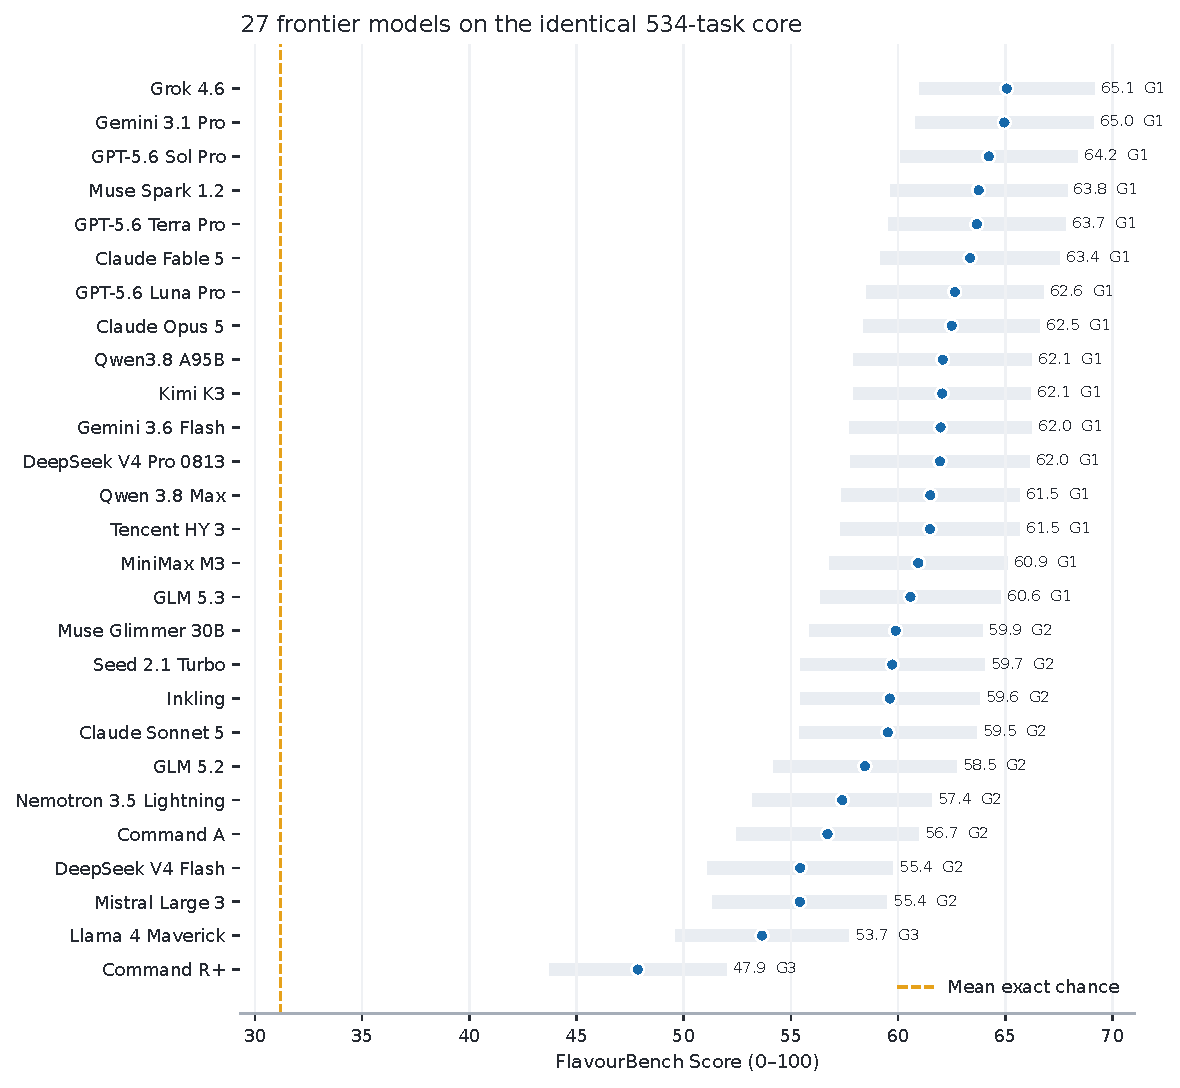
\includegraphics[width=0.92\linewidth]{figures/complete-core/complete-core-leaderboard-forest.pdf}
  \caption{FlavourBench Score with simultaneous 95\% max-$t$ intervals. The letter-free group
  numbers are inferential tiers: a point rank is shown for navigation, while models inside an
  unresolved group should not be read as a statistically established ordering.}
  \label{fig:leaderboard}
\end{figure*}

\begin{table*}[t]
  \centering
  \scriptsize
  \setlength{\tabcolsep}{3.6pt}
  \begin{tabular}{@{}r l r c c c@{}}
\toprule
Rank & Model & FB Score & simultaneous 95\% CI & rank 95\% CI & group \\
\midrule
1 & Grok 4.6 & 65.1 & [61.0, 69.2] & [1, 5] & 1 \\
2 & Gemini 3.1 Pro & 65.0 & [60.8, 69.1] & [1, 6] & 1 \\
3 & GPT-5.6 Sol Pro & 64.2 & [60.1, 68.4] & [1, 8] & 1 \\
4 & Muse Spark 1.2 & 63.8 & [59.6, 67.9] & [1, 10] & 1 \\
5 & GPT-5.6 Terra Pro & 63.7 & [59.5, 67.8] & [1, 11] & 1 \\
6 & Claude Fable 5 & 63.4 & [59.2, 67.5] & [2, 13] & 1 \\
7 & GPT-5.6 Luna Pro & 62.6 & [58.5, 66.8] & [4, 14] & 1 \\
8 & Claude Opus 5 & 62.5 & [58.4, 66.6] & [3, 15] & 1 \\
9 & Qwen3.8 A95B & 62.1 & [57.9, 66.2] & [4, 17] & 1 \\
10 & Kimi K3 & 62.1 & [57.9, 66.2] & [5, 16] & 1 \\
11 & Gemini 3.6 Flash & 62.0 & [57.7, 66.2] & [4, 17] & 1 \\
12 & DeepSeek V4 Pro 0813 & 62.0 & [57.8, 66.1] & [5, 17] & 1 \\
13 & Qwen 3.8 Max & 61.5 & [57.4, 65.6] & [7, 18] & 1 \\
14 & Tencent HY 3 & 61.5 & [57.3, 65.7] & [6, 19] & 1 \\
15 & MiniMax M3 & 60.9 & [56.8, 65.1] & [8, 20] & 1 \\
16 & GLM 5.3 & 60.6 & [56.4, 64.8] & [8, 20] & 1 \\
17 & Muse Glimmer 30B & 59.9 & [55.9, 63.9] & [12, 21] & 2 \\
18 & Seed 2.1 Turbo & 59.7 & [55.4, 64.0] & [12, 22] & 2 \\
19 & Inkling & 59.6 & [55.4, 63.8] & [12, 22] & 2 \\
20 & Claude Sonnet 5 & 59.5 & [55.4, 63.7] & [13, 22] & 2 \\
21 & GLM 5.2 & 58.5 & [54.2, 62.7] & [16, 23] & 2 \\
22 & Nemotron 3.5 Lightning & 57.4 & [53.2, 61.6] & [19, 25] & 2 \\
23 & Command A & 56.7 & [52.5, 60.9] & [20, 25] & 2 \\
24 & DeepSeek V4 Flash & 55.4 & [51.1, 59.7] & [22, 26] & 2 \\
25 & Mistral Large 3 & 55.4 & [51.4, 59.5] & [22, 26] & 2 \\
26 & Llama 4 Maverick & 53.7 & [49.6, 57.7] & [24, 26] & 3 \\
27 & Command R+ & 47.9 & [43.7, 52.0] & [27, 27] & 3 \\
\bottomrule
\end{tabular}

  \caption{The complete automated leaderboard. Every score and every pairwise comparison uses the
  identical \FBTasks{}-task core. Rank intervals come from the anchor-cluster bootstrap; groups
  summarize the Holm-controlled pairwise graph.}
  \label{tab:leaderboard}
\end{table*}

\subsection{Does the ordering replicate on a second task panel?}

The two panel-specific scores use the same frozen metric and \FBTasksPerPanelFamily{} tasks per
family, but disjoint task IDs.
Their model-level Pearson correlation is \FBPanelPearson{} and their rank correlation is
\FBPanelSpearman{}. These are descriptive stability diagnostics, not a model-selection rule; the
primary leaderboard and its uncertainty use both panels and cluster shared ingredient anchors.
\Cref{fig:panel-replication} exposes every model rather than reducing
replication to a single coefficient.

\begin{figure}[t]
  \centering
  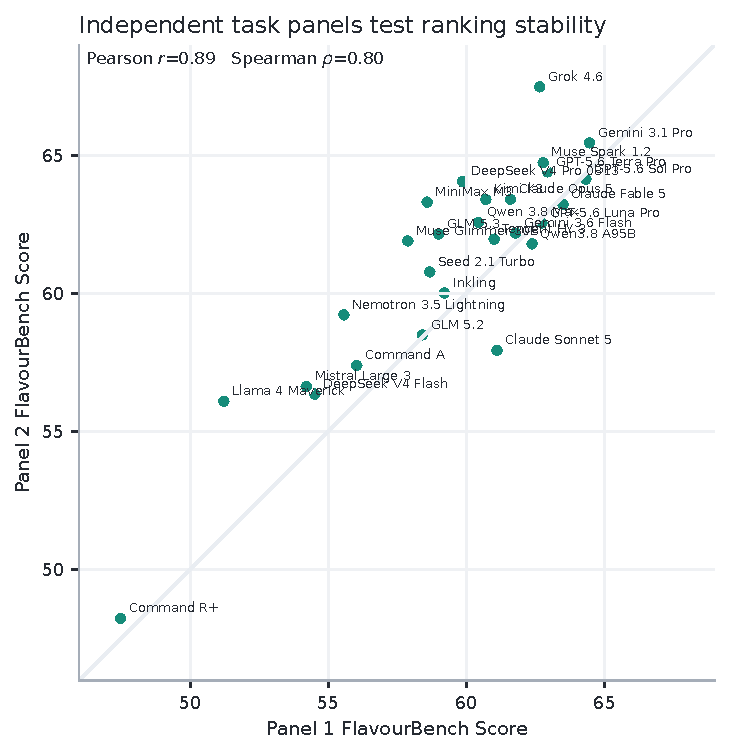
\includegraphics[width=\linewidth]{figures/complete-core/complete-core-panel-replication.pdf}
  \caption{Panel-1 versus panel-2 FlavourBench Score for every endpoint. The diagonal marks exact
  agreement. Each point aggregates \FBTasksPerPanelFamily{} tasks per family; the joint analysis
  uses \FBUniqueAnchors{} unique anchor clusters.}
  \label{fig:panel-replication}
\end{figure}

\subsection{Which pairwise conclusions survive correction?}

The score is continuous, and each model pair is compared on the same \FBTasks{} tasks rather than
on a small number of arena votes. \cref{fig:pairwise} visualizes the
multiplicity-controlled results. Grey cells are scientifically useful: they mark pairs for which
the shared task evidence does not support a directional claim at familywise $\alpha=.05$. This is
different from declaring the two models equal.

\begin{figure}[t]
  \centering
  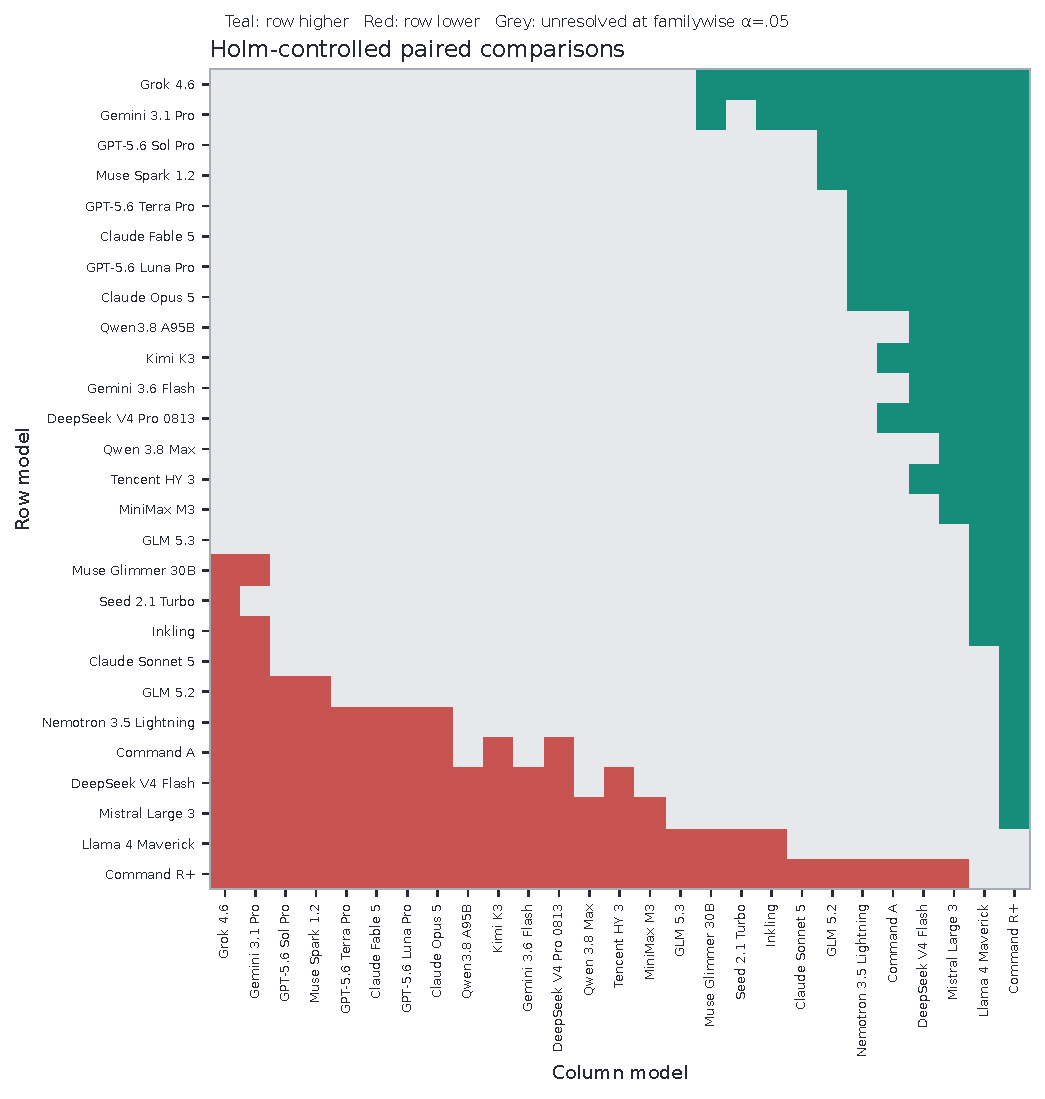
\includegraphics[width=\linewidth]{figures/complete-core/complete-core-pairwise-matrix.pdf}
  \caption{All paired model contrasts after Holm correction. Teal means the row model scores
  higher; red means lower; grey is unresolved.}
  \label{fig:pairwise}
\end{figure}

\subsection{Aggregate scores conceal different culinary profiles}

Family-level results in \cref{fig:families} show that similar aggregate scores can arise from
different strengths. Constraint tasks penalize infeasible portfolios directly, while pairing and
substitution reward graded semantic structure. The three columns are related but not
interchangeable.

\begin{figure}[t]
  \centering
  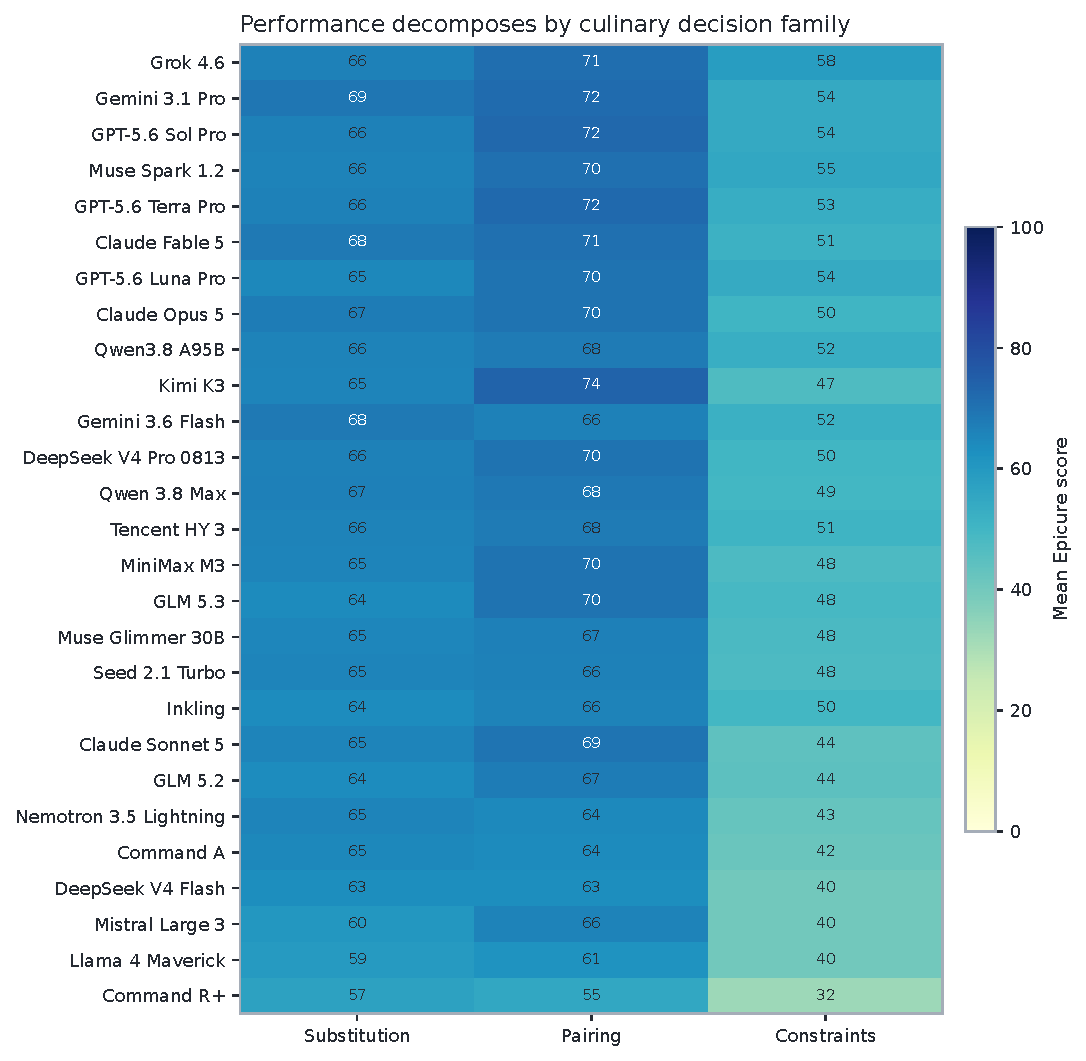
\includegraphics[width=\linewidth]{figures/complete-core/complete-core-family-heatmap.pdf}
  \caption{Mean score by family on the common core. Each family contributes
  \FBTasksPerFamily{} tasks per model. Values share the 0--100 scale but retain family-specific
  decision semantics.}
  \label{fig:families}
\end{figure}

\subsection{Rank uncertainty is visible, not hidden}

Bootstrap rank intervals expose how often small score differences change order under plausible
resampling of ingredient anchors. \Cref{fig:rank-intervals} separates stable regions of the table
from visually tempting but statistically unsupported micro-ranks. This is stricter than sorting
point estimates and printing an ordinal list without uncertainty.

\begin{figure}[t]
  \centering
  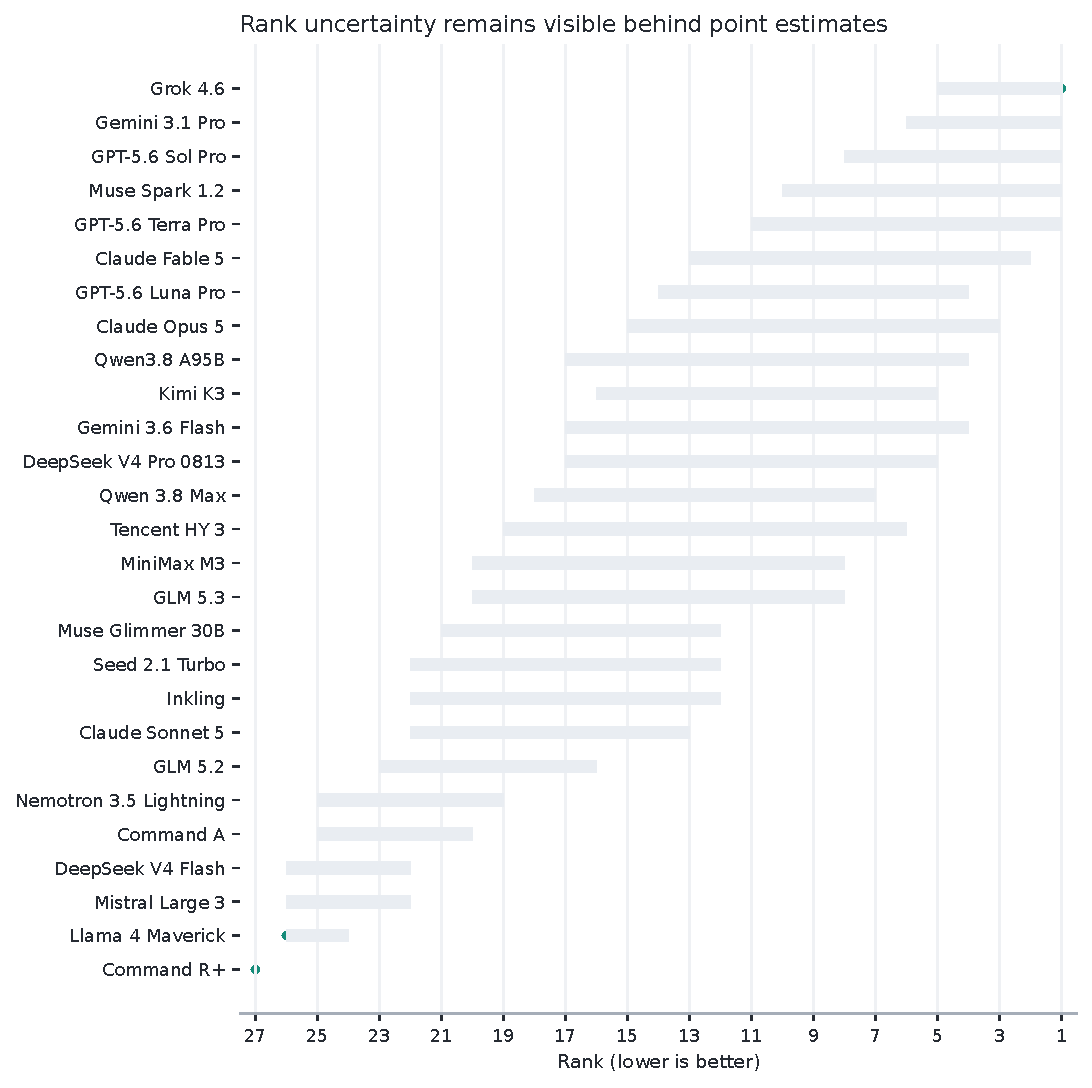
\includegraphics[width=\linewidth]{figures/complete-core/complete-core-rank-intervals.pdf}
  \caption{Point rank and 95\% bootstrap rank interval for every endpoint. Narrow intervals imply
  a stable location; overlapping intervals mark unresolved local order.}
  \label{fig:rank-intervals}
\end{figure}

\subsection{Real prompts and model decisions}

\Cref{tab:examples} reports one deterministically selected common-core task from each family with
responses from the highest- and lowest-point-estimate endpoints. Selection follows a fixed hash
rule rather than task score. The public
case-study JSON contains the complete prompt, all eight choices, the
optimal portfolio, both raw model responses, selected ingredient identities, and exact scores.
The examples illustrate why continuous scoring is preferable to exact match: two non-optimal
portfolios can differ substantially in culinary utility.

\begin{table*}[t]
  \centering
  \scriptsize
  \setlength{\tabcolsep}{3pt}
  \begin{tabularx}{\linewidth}{@{}l X X X@{}}
\toprule
Family & Prompt & Higher-ranked selection & Lower-ranked selection \\
\midrule
Substitution & Select three alternatives to `boursin cheese` that best preserve its dairy role, regional context, and mutual portfolio coherence. & caciocavallo, fromage blanc, grana padano (100) & fromage blanc, quail egg, goose egg (15) \\
Pairing & Select the three-ingredient bundle with the strongest learned pairing to `sweetbread` and the best internal coherence. & parsnip, cipollini onion, porcini mushroom (92) & parsnip, pickled onion, peppadew pepper (0) \\
Constraints & For a dish centered on `potato`, select three vegetarian complements with NOVA processing level at most 2; among valid portfolios, maximize learned pairing and coherence. & parsley, black pepper, thyme (100) & cheese, bay leaf, parsley (0) \\
\bottomrule
\end{tabularx}

  \caption{Three common-core response examples. Parentheses give the fixed task score. The complete
  prompts and unabridged responses are released in machine-readable form.}
  \label{tab:examples}
\end{table*}

\section{From benchmark to training signal}
\label{sec:training}

The exhaustive task map makes \system{} useful beyond a static leaderboard. For a task state
$x_t$ and selected portfolio $a$, \epicure{} supplies a deterministic reward $r(x_t,a)=s_t(a)$.
This creates three immediate training interfaces:
\begin{enumerate}[label=\arabic*.]
  \item supervised learning from the optimal portfolio and the full ordering of 56 candidates;
  \item preference or contrastive learning from any pair $(a_i,a_j)$ with known reward difference;
  \item offline or online policy optimization using dense bounded rewards and held-out anchors.
\end{enumerate}

The present experiment evaluates models rather than training them. The release supplies the
environment, reward function, and anchor identifiers required for a clean next experiment: train
on development reward maps and measure transfer on disjoint held-out anchors. Direct optimization
on the public test map would measure memorization rather than culinary learning.

\section{Reproducibility}
\label{sec:reproducibility}

The release is organized around content-addressed inputs and append-only outputs. It includes:
\begin{itemize}
  \item both exact content-addressed task sets (\FBTasks{} scheduled tasks and
  \FBUniqueAnchors{} unique anchors), with prompts, candidates, all 56 portfolio scores, oracle
  provenance, task strata, and task-set digests;
  \item the \FBModels{}-model manifest, exact provider route per model, fallback policy, supported
  parameters, endpoint contract, and route digest;
  \item all response records used to construct the \FBCompleteCells{}-cell ranked matrix,
  including raw text, completion state, usage, latency, parser output, task score, and digest;
  \item all content-addressed provider-attempt events referenced by those responses, including
  normalized and native finish reasons used to distinguish refusals from ordinary completions;
  \item the frozen joint analysis plan, anchor-cluster contract, seeds, 50,000 bootstrap and
  100,000 sign-flip counts, all \FBPairs{} pairwise rows, cross-panel diagnostics, and the final
  statistical release; and
  \item a verifier and asset builder that reconstruct the leaderboard CSV, pairwise CSV, LaTeX
  tables, and vector figures from local files without provider access.
\end{itemize}

Responses are written once under a model slot and cell identifier. Existing valid cells are
skipped on resume; conflicting artifacts fail closed. Provider fallback is disabled, so the route
shown in the manifest is the route measured. The task maps and analysis plan were frozen before
the clean primary lineage; transport-calibration responses are retained separately and never enter
the leaderboard.

\section{Related work}

General-purpose evaluation spans broad suites such as HELM \cite{liang2022helm}, difficult
knowledge tests such as MMLU-Pro and GPQA \cite{wang2024mmlupro,rein2023gpqa}, live contamination-
resistant sets \cite{white2024livebench,jain2024livecodebench}, and human preference systems such
as Chatbot Arena \cite{chiang2024chatbotarena}. Model judges increase scale but introduce their own
bias and calibration problems \cite{zheng2023judging}. \system{} instead takes the executable-
environment route used by software and agent benchmarks: SWE-bench runs repository tests
\cite{jimenez2023swebench}, BFCL evaluates function calls \cite{patil2025bfcl}, and $\tau$-bench
checks interaction outcomes against database state \cite{yao2024taubench}.

Culinary datasets and benchmarks cover ingredient networks, recipe understanding, planning,
nutrition, and food knowledge \cite{ahn2011flavor,garg2018flavordb,salvador2017recipe1m,
choi2024cookingsense,wu2025recipe2plan,hua2025nutribench,eftimov2026foodbench,jin2026diningbench}.
Our focus is narrower and complementary: common-task frontier model measurement against a
versioned culinary decision environment, with exhaustive partial-credit maps and paired inference.

\section{Limitations}

FlavourBench Score measures agreement with one published \epicure{} release, not universal human
taste. Within-task min--max normalization makes the 0--100 scale comparable while discarding
absolute raw-utility magnitudes. The tasks evaluate constrained ingredient selection rather than
full recipe generation, sensory execution, safety advice, or long-horizon kitchen planning. The
common-core requirement removes differential missingness from ranking, but it also restricts the
estimand to tasks completed by every endpoint; the released supplemental tracks retain the rest.
Results bind particular model routes and collection dates. The dense reward surface supports
learning experiments, but this paper does not test whether optimizing \epicure{} reward transfers
to human cooking outcomes.

\section{Conclusion}

\system{} makes culinary reasoning measurable without asking one language model to grade another.
A versioned runtime enumerates every candidate decision, a \FBModels{}-model complete panel
produces one continuous score, and paired uncertainty distinguishes resolved differences from
apparent rank order. The result is an automated leaderboard that can be rerun, audited, and used
as a dense training environment. Under this executable culinary ground truth and the released
\FBTasks{}-task, \FBUniqueAnchors{}-cluster distribution, every score, interval, contrast, and
figure is reconstructable from public artifacts.

\bibliographystyle{plain}
\bibliography{references}

\clearpage
\onecolumn
\appendix
\section{Exact execution routes}
\label{app:routes}

\begin{center}
  \centering
  \scriptsize
  \setlength{\tabcolsep}{4pt}
  \begin{tabular}{@{}l l l l@{}}
\toprule
Model & Backend & Panel 1 route & Panel 2 route \\
\midrule
Grok 4.6 & openrouter & xai/zdr & xai/zdr \\
Gemini 3.1 Pro & openrouter & google-ai-studio & google-ai-studio \\
GPT-5.6 Sol Pro & openrouter & openai/flex & openai/flex \\
Muse Spark 1.2 & openrouter & meta & meta \\
GPT-5.6 Terra Pro & openrouter & openai/flex & openai/flex \\
Claude Fable 5 & openrouter & google-vertex/global & google-vertex/global \\
GPT-5.6 Luna Pro & openrouter & openai/flex & openai \\
Claude Opus 5 & openrouter & azure/us & azure/us \\
Qwen3.8 A95B & openrouter & alibaba & alibaba \\
Kimi K3 & openrouter & morph & morph \\
Gemini 3.6 Flash & openrouter & google-vertex/us & google-vertex/us \\
DeepSeek V4 Pro 0813 & openrouter & gmicloud/fp8 & gmicloud/fp8 \\
Qwen 3.8 Max & openrouter & alibaba & alibaba \\
Tencent HY 3 & openrouter & gmicloud/bf16 & gmicloud/bf16 \\
MiniMax M3 & openrouter & venice/fp8 & venice/fp8 \\
GLM 5.3 & zai\_coding\_direct & zai-coding-plan-direct & zai-coding-plan-direct \\
Muse Glimmer 30B & openrouter & fireworks & fireworks \\
Seed 2.1 Turbo & openrouter & seed/fp8 & seed/fp8 \\
Inkling & openrouter & deepinfra/fp8 & deepinfra/fp8 \\
Claude Sonnet 5 & openrouter & amazon-bedrock/claude-on-aws & amazon-bedrock/claude-on-aws \\
GLM 5.2 & openrouter & coreweave/fp4 & coreweave/fp4 \\
Nemotron 3.5 Lightning & openrouter & venice/fp4 & venice/fp4 \\
Command A & openrouter & cohere & cohere \\
DeepSeek V4 Flash & openrouter & deepinfra/fp4 & deepinfra/fp8 \\
Mistral Large 3 & openrouter & mistral & mistral \\
Llama 4 Maverick & openrouter & digitalocean & digitalocean \\
Command R+ & openrouter & cohere & cohere \\
\bottomrule
\end{tabular}

  \captionof{table}{Frozen execution routes by panel. Automatic fallback is disabled; route
  differences indicate complete, score-blind model-block replacements rather than cell pooling.}
\end{center}

\section{Per-family scores}

\begin{center}
  \centering
  \scriptsize
  \setlength{\tabcolsep}{4pt}
  \begin{tabular}{@{}l r r r@{}}
\toprule
Model & Substitution & Pairing & Constraints \\
\midrule
Grok 4.6 & 66.1 & 70.9 & 58.2 \\
Gemini 3.1 Pro & 69.0 & 71.6 & 54.2 \\
GPT-5.6 Sol Pro & 66.2 & 72.5 & 54.1 \\
Muse Spark 1.2 & 65.9 & 70.3 & 55.0 \\
GPT-5.6 Terra Pro & 66.1 & 72.1 & 52.8 \\
Claude Fable 5 & 68.2 & 70.6 & 51.3 \\
GPT-5.6 Luna Pro & 64.5 & 69.7 & 53.7 \\
Claude Opus 5 & 67.2 & 69.9 & 50.4 \\
Qwen3.8 A95B & 66.0 & 67.8 & 52.5 \\
Kimi K3 & 65.5 & 73.7 & 47.0 \\
Gemini 3.6 Flash & 68.1 & 66.2 & 51.6 \\
DeepSeek V4 Pro 0813 & 66.4 & 69.5 & 49.9 \\
Qwen 3.8 Max & 66.6 & 68.5 & 49.5 \\
Tencent HY 3 & 66.0 & 67.9 & 50.5 \\
MiniMax M3 & 65.4 & 69.9 & 47.6 \\
GLM 5.3 & 63.7 & 69.6 & 48.4 \\
Muse Glimmer 30B & 65.1 & 66.8 & 47.8 \\
Seed 2.1 Turbo & 65.3 & 66.2 & 47.6 \\
Inkling & 63.6 & 65.8 & 49.5 \\
Claude Sonnet 5 & 65.3 & 69.2 & 44.1 \\
GLM 5.2 & 63.6 & 67.2 & 44.5 \\
Nemotron 3.5 Lightning & 65.3 & 64.3 & 42.5 \\
Command A & 64.7 & 63.9 & 41.6 \\
DeepSeek V4 Flash & 63.1 & 63.2 & 40.1 \\
Mistral Large 3 & 60.4 & 65.8 & 40.0 \\
Llama 4 Maverick & 59.4 & 61.4 & 40.2 \\
Command R+ & 56.7 & 54.9 & 32.0 \\
\bottomrule
\end{tabular}

  \captionof{table}{Mean score in each \FBTasksPerFamily{}-task family. Every entry uses the same
  tasks for every model; the equal-family mean is the FlavourBench Score.}
\end{center}

\section{Protocol constants}

\begin{center}
  \centering
  \footnotesize
  \begin{tabular}{@{}l r@{}}
    \toprule
    Quantity & Frozen value \\
    \midrule
    Models & \FBModels{} \\
    Collection panels & \FBPanelCount{} \\
    Primary tasks per model & \FBTasks{} \\
    Unique anchor clusters & \FBUniqueAnchors{} \\
    Tasks per family & \FBTasksPerFamily{} \\
    Candidate ingredients & 8 \\
    Selected ingredients & 3 \\
    Scored portfolios per task & 56 \\
    Complete response cells & \FBCompleteCells{} \\
    Bootstrap replicates & \FBBootstrapResamples{} \\
    Sign-flip replicates & \FBPermutationResamples{} \\
    Pairwise hypotheses & \FBPairs{} \\
    Shared cells per pair & \FBTasks{} \\
    Common-core rule & Status/parser only; score-blind \\
    \bottomrule
  \end{tabular}
  \captionof{table}{Core design and inference constants fixed before clean primary execution.}
\end{center}

\end{document}
